\section{Raspberry Pi}
Der Raspberry Pi stellt in diesem Projekt unter anderem die Schnittstelle zum Web oder Internet dar. Für den Raspberry Pi sprachen einige Argumente.
\begin{itemize}
\item Es kann das gleiche Funkmodul wie für die Arduinos verwendet werden
\item Es ist eine große Community vorhanden
\end{itemize}
Ferner handelt es sich beim Raspberry Pi um einen Ein-Platinen-Rechner. 

\subsection{Hardware}
Bei dem Hauptprozessor des Raspberry Pi handelt es sich um einen Broadcom BCM2835. Die Architektur des Prozessors nennt sich \textit{ARM}. ARM hat einige Vorteile gegenüber x86 Prozessoren: 
\begin{itemize}
\item kleiner Energiebedarf
\item geringe Wärmeentwicklung
\subitem normalerweise keine Kühlung notwendig
\item kleine Bauweise
\end{itemize}

\subsubsection{Allgemein}
Die ARM-Architektur besitzt folgende Eigenschaften: 
\begin{itemize}
\item \ac{RISC}
\item 32-Bit Daten- und Adressbus
\item 7 Prozessor Modi
\item 37 Register
\item 5 Hauptadressierungsmodi
\item Datentypen
\subitem 32 Bit Wort
\subitem 16 Bit Halbwort
\subitem Byte (8 Bit)
\item Instruktionen
\subitem 54 ARM-Instruktionen, sie sind jeweils ein Wort
\subitem 38 Thumb-Instruktionen
\subitem Datenverarbeitungen werden auf Wörter angewandt
\end{itemize}

\subsubsection{Modi}
\begin{table}
    \begin{tabular}{lll}
    Modus          & Beschreibung                    & Ausnahme-Modus? \\ \hline
    User           & Ausführung normaler Programme   & nein            \\
    System         & privelegierter Modus            & nein            \\
    Supervisor     & Modus für Systemcalls           & ja              \\
    Abort          & Memory Abort                    & ja              \\
    Undefined      & Undefinierte Anweisung (Fehler) & ja              \\
    Interrupt      & Modus für Interrupts            & ja              \\
    Fast Interrupt & Modus für schnellen Interrupt   & ja              \\
    \end{tabular}
    \caption {ARM-Modi}
\end{table}
Ein Interrupt und ein Fast Interrupt unterscheiden sich in ihrer Priorität. Ein Fast Interrupt kann also einen Interrupt unterbrechen. Es darf jedoch nur ein Fast Interrupt zu einem Zeitpunkt auftreten. Der User-Modus ist der einzige Modus ohne Privilegien, die anderen Modi haben mehr Rechte wie der User-Modus. In User-Modus werden standardmäßig Programme ausgeführt. Einige Register sind Modussensitiv, soll heißen, dass sie nur in einem bestimmten Modus nutzbar sind. Wenn der Rechner startet, befindet sich der Prozessor im Supervisor-Modus. Später kann von jedem Modus aus gewechselt werden, außer aus dem User-Modus. Man kann ihn nur über einen Softwareinterrupt verlassen. 
\subsubsection{Register}
Im User-Modus kann man über die Register R0 bis R12 frei verfügen. Register R13 ist der Stackpointer, Register R14 das Linkregister. Das Linkregister merkt sich die Return-Adresse um nach einem Funktionsaufruf zurückzukehren. Das Register R15 ist wird als Programm-Counter genutzt.

\begin{figure}
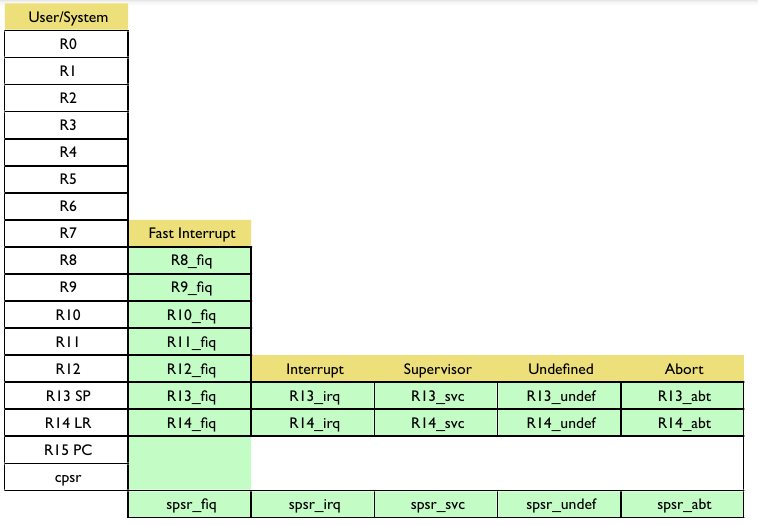
\includegraphics[width=\columnwidth]{bilder/overviewRegister} 
\caption{Überblick über die Register Quelle: arm-2009.pdf}
\label{Register}
\end{figure}

Das Statusregister ist im Detail wie folgt aufgebaut:
\begin{figure}
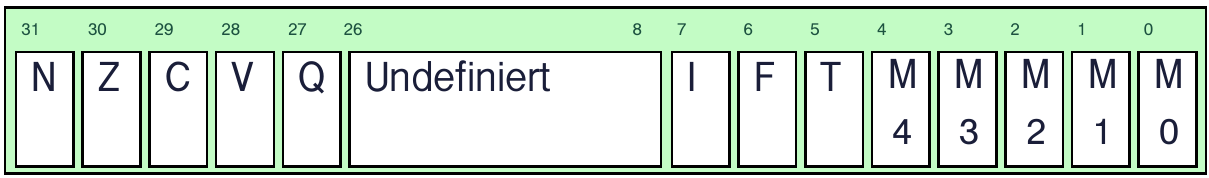
\includegraphics[width=\columnwidth]{bilder/statusRegister} 
\caption{Das Statusregister im Detail Quelle: arm-2009.pdf}
\label{Statusregister}
\end{figure}
 
Das hochwertigste Bit fungiert als Vorzeichen. Das 30. Bit ist bei Null gesetzt, das 29. Bit \textit{C} ist gesetzt, wenn das Ergebnis einer Operation eine Übertrag hat. Bit \textit{V} ist bei einem Overflow (Überlauf) gesetzt. Bit \textit{Q} fungiert bei ARM-Prozessoren, die als \ac{DSP} eingesetzt werden, als Überlaufbit für erweiterte Instruktionen. Die Bits 26 bis 8 sind undefiniert, Bit \textit{I} (7) ist das Interruptbit. Es ist bei einem Interrupt gesetzt. Bit \textit{F} (6) ist das Fast Interrupt-Bit. Es ist dementsprechend gesetzt. Das Bit \textit{T} (5) gibt den zeigt an, ob der Thumb-Mode aktiv ist. Im Thumb-Mode sind die Instruktionen nicht 32 Bit lang, sondern nur 16 Bit. Instruktionen im Thumb-Mode sind bieten demnach weniger Optionen. Sie arbeiten häufig implizit. Der Vorteil von Thumb-Instruktionen ist, dass die Instruktionen weniger Speicher benötigen. Die Abarbeitngsgeschwindigkeit von 32 Bit Instruktionen und Thumb-Instruktionen ist identisch. Die Bits 4 bis 0 kodieren den Modus der CPU:
\begin{table}
    \begin{tabular}{l|l}
    Bit M\textsubscript{4}, ..., M\textsubscript{0}  & Modus          \\ \hline
    10000 & User           \\
    10001 & Fast Interrupt \\
    10010 & Interrupt      \\
    10011 & Supervisor     \\
    10111 & Abort          \\
    11011 & Undefined      \\
    11111 & System         \\
    \end{tabular}
    \caption {Modi im ARM Statusregister}
\end{table}
%TODO Quelle: arm-2009.pdf

\subsubsection{Exceptions}
Der ARM-Prozessoren kennen typischer sieben verschiedene Exceptions (Ausnahmen). Sie haben folgende Priorität:
\begin{enumerate}
\item Reset
\item Data Abort
\item Fast Interrupt Request
\item Interrupt Request
\item Prefetch Abort
\item Undefined Instruction
\setcounter{enumi}{5} %% folgendes item soll (auch) die nummer 6 haben
\item Software Interrupt
\end{enumerate}

Kommt es zur Exception \textit{Reset}, bricht der Prozessor seine Arbeit an der momentanen Stelle ab und springt sofort zur Adresse, die der Reset-Exception zugeteilt ist. Diese Adresse der Speicherstelle an die der Prozessor nach dem Start springt, ist mit der Reset-Adresse identisch. 
Greift ein Programm unberechtigterweise auf einen Speicherbereich zu, schmeißt der schmeißt das System die \textit{Data Abort}-Exception. Anschließend springt der Prozessor an eine definierte Speicherstelle. Hier kann der Programmierer die Exception durch Implementieren einer Routine abfangen. Ein \textit{Fast Interrupt Request} führt zur Abarbeitung der entsprechenden Methode wenn die Anfrage gültig ist, das heißt wenn der Prozessor gerade keine andere Exception und der Fast Interrupt Request eindeutig ist. Gleiches wie für den Fast Interrupt Request gilt auch für den Interrupt Request. Allerdings kann der hat der Interrupt Request eine niedrigere Priorität. Der Prozessor kann ihn nur behandeln, wenn keine Exception höherer Priorität auftritt. Dies kann beispielsweise ein Fast Interrupt Request sein. Externe Hardware kann ein (Fast) Interrupt Request auslösen. 
Will der Prozessor beim Fetch auf eine Adresse zugreifen, auf die er kein Zugriff hat, so schmeißt er eine \textit{Prefetch Abort}-Exception. Kennt der Prozessor die geforderte Instruktion nicht, so kommt es zu eines \textit{Undefined Instruction}-Exception. Sie hat die gleiche Priorität wie die \textit{Software Interrupt}-Exception. Dies hat den Hintergrund, dass es nicht möglich ist, dass sie gleichzeitig auftreten. In einem Programm kann man explizit eine \textit{Softtware Interrupt} Exception auslösen.    


%TODO Quelle: arm-2009.pdf 

\subsubsection{Memory Management Unit}
ARM-Prozessoren verfügen wie auch x86-Prozessoren über eine \ac{MMU}. Dieser Hardware-Baustein hat die Aufgabe virtuelle Speicheradressen in reale Speicheradressen zu übersetzten. Dies hat mehrere Vorteile: 
\begin{itemize}
\item einfacherer Umgang mit Adressen
\item Erhöhung der Sicherheit 
\item keine großen, ungenutzten Speicherstellen am Stück 
\end{itemize}

\begin{figure}
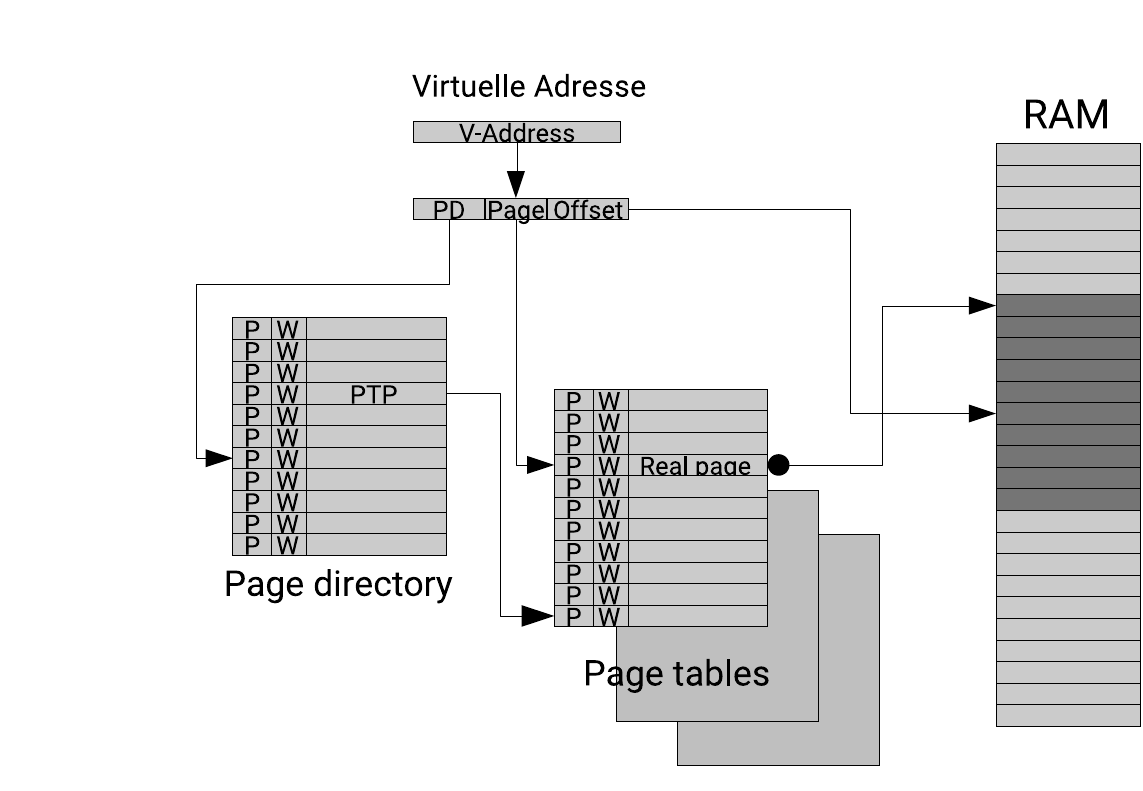
\includegraphics[scale=0.3]{bilder/mmu} 
\caption{Virtuelle Adressierung Quelle: Richter}
\label{MMU}
\end{figure}

Die Virtuelle Adresse (V-Address) besteht (vereinfacht) aus einer Adresse für das Page Directory, der Adresse für die eigentliche Page und dem Offset innerhalb der Page. \textit{P} und \textit{W} in der Abbildung sind Bits. Ist das \textit{P}-Bit gesetzt, so ist die jeweilige Seite im Hauptspeicher verfügbar. Ist das \textit{W}-Bit gesetzt, so darf auf die Page geschrieben werden. Das \textit{W}-Bit ist für weitere Mechanismen notwendig. Diese sind jedoch nicht Gegenstand dieser Arbeit.  

Dadurch, dass der Prozessor nicht mit realen Adressen arbeiten muss, muss der Programmierer oder Compiler die konkreten realen Adressen nicht kennen. Nun ist es möglich zu realisieren, dass es für Programme so aussieht, als wäre der zugeteilte Speicherbereich am Stück. Physikalisch ist der zugewiesene Speicher jedoch über den ganzen RAM verteilt. Ferner ist es auch der Fall, dass ein Betriebssystem ständig Programme startet und beendet. Endet ein Programm, so muss man den allokierten   Speicherbereich wieder dellokieren. Die virtuelle Adressierung verhindert in diesem Zusammenhang, dass groß Speicherbereiche "brach" liegen. Würde man kein virtuelle Adressierung verwenden, so ist nach dem Ende eines Programmes, dass 1 Gb Speicher benutzt hat, eine 1 Gb große Lücke im Speicher. Dieser Umstand kann zu Problemen führen, wenn ein neues Programm startet und viel Speicher benötigt. Im Falle der virtuellen Adressierung ist es irrelevant, ob der angeforderte Speicher am Stück ist oder ob die benutzen Speicherstellen über den RAM verteilt sind.    

%TODO Quelle: Richter

\subsubsection{Externe Anschlüsse}
Der Raspberry Pi verfügt über mehrere physikalische Schnittstellen. 
\begin{itemize}
\item \ac{GPIO}
\item USB
\item 3,5 mm Klinke für Audio
\item \ac{CSI}
\item RJ45 für Ethernet
\item HDMI
\item \ac{DSI}
\end{itemize}

Die \ac{GPIO}-Pins ermöglichen unter anderem eine Kommunikation über \ac{I2C} und den \ac{SPI}. 

\subsubsection{\ac{I2C}} Bei \ac{I2C} handelt es sich um einen seriellen Bus mit zwei Leitungen. Es gibt die Leitung SCL (Signal Clock) und SDA (Signal Data). Da mit SCL eine Taktleitung vorhanden ist, redet man von einem synchronen Bus. Der Bus arbeitet nach dem Master/Slave-Prinzip. Er ist des Weiteren auch Multi-Master-fähig. Es können mehere Teilnehmer die Rolle des Masters einnehmen. Prinzipiell können Master zwei Operationen durchführen: 
\begin{itemize}
\item Lesen
\item Schreiben
\end{itemize} 
Um einen reibungslosen Ablauf zu gewährleisten, organisiert sich der Bus durch
\begin{itemize}
\item Startbedingung
\item Stoppbedingung
\item Acknowledge
\item No-Acknowledge
\end{itemize}
Bevor ein Master mit einer Operation beginnen kann, muss er prüfen, ob dieser frei ist. Ist der Bus frei, so sind beide Leitungen auf HIGH (fünf Volt). 

%TODO : i2c_frei

Nun kann der Master seine Transaktion mit der Startbedingung ankündigen. Dazu lässt er die Taktleitung SCL auf HIGH und legt die Datenleitung über einen Pull-down-Widerstand auf Masse (LOW). Diese Vorgehensweise ermöglicht die Mult-Master-Fähigkeit. Möchte jetzt ein weiterer Master eine Übertragung an diesem Bus starteten, so fällt ihm bei Prüfen des Busses auf, dass SDA LOW ist. An dieser Tatsache kann er auch nichts ändern. Der Strom fließt über den Pull-down-Widerstand des aktiven Masters auf Masse ab. Nur der aktive Master kann SDA wieder auf HIGH legen und den Bus damit wieder frei geben.  

%TODO : i2c_start

Daten sind wie folgt kodiert: Für eine logische Null zieht der entsprechende Teilnehmer die Datenleitung (SDA) auf LOW. In der Zeit, in der die Taktleitung HIGH ist, gilt die logische Null. 

%TODO : i2c_0

Für eine logische Eins läßt der Busteilnehmer die Datenleitung auf HIGH. Auch die logische Eins gilt so lange, bis SCL HIGH ist. 

%TODO : i2c_1

Nur ein Master kann eine Operation starten mittels Startbedingung (sofern der Bus frei ist). Nach dem ein Master eine den Bus erfolgreich reserviert hat, schreibt er ein Byte auf die Leitung. Die ersten 7 Bit des Bytes sind eine Adresse. Sie gehört dem Slave, mit dem der Master kommunizieren möchte. Bei \ac{I2C}  kann man somit 128 verschiedene Adressen vergeben. Das letzte Bit von dem Byte gibt die Richtung des Informationsflusses an. Der Master kann entweder lesen (1) oder schreiben (0). Diesem ersten Byte lauschen alle Geräte. Erkennt ein Slave seine Adresse auf dem Bus und er ist verfügbar, so sendet er ein Acknowledge.

%TODO i2c_ack

Erkennt ein Gerät seine Adresse, ist aber nicht verfügbar, so sendet es ein No-Acknowledge.

%TODO i2c-noAck

Um eine Übertragung zu beenden, zieht der Master die Datenleitung auf LOW, die Taktleitung bleibt währenddessen auf HIGH. 

%TODO Bilder: http://www.cc-zwei.de/wiki/index.php?title=I2C_Bus_Hintergrundwissen

%TODO Quelle: Rasi Handbuch, VL Lehmann

\subsubsection{\ac{SPI}}
Bei \ac{SPI} kann man relativ hohe Datenübertragungsraten erreichen. Dazu darf allerdings die Wegstrecke der Leitungen nur relativ klein sein (auf einem Chip). Die Spezifikation von \ac{SPI} ist weiter gefasst als die von \ac{I2C}. Ferner handelt es sich bei \ac{SPI} um kein Bussystem im klassischen Sinne. Jedes Gerät benötigt nämlich unter anderem eine eigene Leitung. Auch eine exakte Spezifikation der Geräte sieht \ac{SPI} nicht vor. 

%TODO Bild spi einfügen, Quelle rapi Handbuch

Es folgt eine Beschreibung, wie die \ac{SPI}-Kommunikation beim Raspberry Pi aussehen kann: Der Master legt einen Takt von 100 kHz auf die Taktleitung SCK. Nun selektiert er über eine Slave-select-Leitung (SS) einen Slave. Die SS-Leitung ist LOW-aktiv. Das heißt, dass die Leitung im unselektierten Zustand HIGH ist, im selektierten Zustand ist sie LOW. 

 




%TODO Quelle: Rasi Handbuch, VL Lehmann
 
\subsection{Software}
Dieses Unterkapitel betrachtet die 
 
%TODO Exceptions und Assembler hier (aus arm-200)





          
 
